\subsection{Cross-event mechanism and closed-loop performance}
\label{sec:res-performance}

\subsubsection{Cross-event recovery mechanism and theoretical checks}
\label{sec:res-mech}

Two events are considered first: a preceding event A from 17:00 and a subsequent event B that starts after a gap
$\tau$. \figref{fig:mech} compares the maximum sustainable reduction $\Gamma_B$ of event B with its stand-alone
capability $\Gamma_B^0$, and \tabref{tab:mech} lists the case with A = 6~MW $\times$ 2~h, B = 1~h and $\gamma=1.10$.
When event A ends, the backlog energy is 4.9~MWh, the storage deficit 12.3~MWh and $\Gamma_B^0\approx8.0$~MW.

\begin{figure*}[!t]
\centering
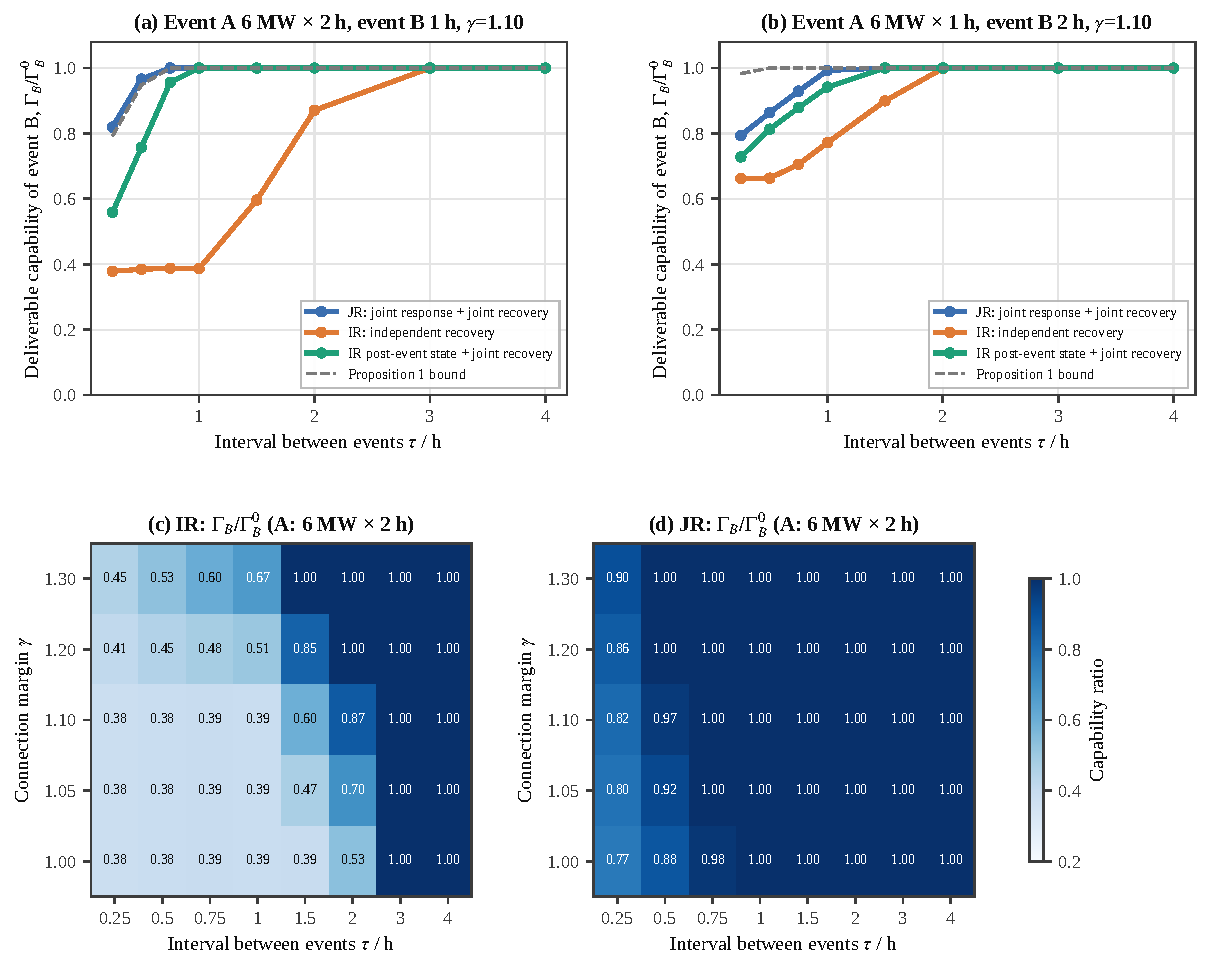
\includegraphics[width=0.84\textwidth]{fig02_mechanism.pdf}
\caption{Cross-event recovery mechanism. (a)(b) Deliverable capability of event B relative to its stand-alone capability
versus the gap ($\gamma=1.10$); (c)(d) capability ratio of independent and joint recovery on the gap--margin plane
(event A: 6~MW $\times$ 2~h).}
\label{fig:mech}
\end{figure*}

\begin{table}[!t]
\caption{Deliverable capability ratio $\Gamma_B/\Gamma_B^0$ (event A 6~MW $\times$ 2~h, event B 1~h, $\gamma=1.10$).}
\label{tab:mech}
\centering\footnotesize
\setlength{\tabcolsep}{3.3pt}
\begin{tabular}{@{}cccccc@{}}
\toprule
Gap $\tau$ (h) & $H$ (MWh) & IR & \makecell{IR state +\\joint recovery} & \makecell{JR (joint response\\and recovery)} & \makecell{Bound of\\Prop.~\ref{prop:bound}}\\
\midrule
0.25 & 1.65 & 0.38 & 0.56 & 0.82 & 0.79\\
0.50 & 3.28 & 0.38 & 0.76 & 0.97 & 0.95\\
0.75 & 4.91 & 0.39 & 0.96 & 1.00 & 1.00\\
1.00 & 6.55 & 0.39 & 1.00 & 1.00 & 1.00\\
1.50 & 9.80 & 0.60 & 1.00 & 1.00 & 1.00\\
2.00 & 13.02 & 0.87 & 1.00 & 1.00 & 1.00\\
\bottomrule
\multicolumn{6}{@{}p{0.97\columnwidth}@{}}{\scriptsize The bound is evaluated at the post-event state of IR, so JR, which also changes the response in event A, may exceed it.}
\end{tabular}
\end{table}

Independent recovery must repay the whole debt before it can respond again: for gaps of up to 1~h, event B retains
only 38--39\% of its stand-alone capability, and 87\% is reached only after 2~h. Joint recovery repays only what the
next event needs. From the same post-event state, a gap of 0.75~h, whose channel energy is only 29\% of the total debt,
already restores 96\%; if the preceding response is planned jointly as well, 0.5~h suffices for 97\%. When event B is
longer (A 1~h, B 2~h), the energy-type limit becomes more prominent: for $\tau\le1$~h, IR reaches 0.66--0.77, joint
recovery from the IR state 0.73--0.94 and JR 0.79--0.99.

The bound of Proposition~\ref{prop:bound} holds in all 80 cases, never exceeding the optimal value from the same
post-event state, and is within 0.05~MW of it in 47 cases; the looser cases occur for $\tau\le0.5$~h, where the
channel width, charging power and EDF order cannot be shifted freely in time while $H$ counts only the total. The
closed form of Theorem~\ref{thm:closed} agrees with the discrete-time LP in all 68 stylised cases to within
$1\times10^{-5}$~MW (\figref{fig:theorem}). With $p_f=5$~MW, $X=5$~MWh and $h=3$~MW, the minimum full-recovery gaps of
IR and JR differ by 0, 0.83, 1.67 and 1.67~h for $L$ = 1, 1.5, 2 and 3~h, exactly $\min(X,p_f(L-D_B))/h$, and joint
recovery has no value when $L=1$~h equals the duration of event B, as predicted by Corollary~\ref{cor:novalue}(a).

\subsubsection{Case-day comparison under identical commitments}
\label{sec:res-caseday}

All strategies are run in closed loop with 15-min steps, the same commitments, SLA and physical constraints, and are
settled by the Jiangsu rules (\tabref{tab:caseday}). Two commitments are used. The coupled day-ahead commitment is
3.27/6.65/7.90~MW for $\crb=3$: because E3 is paid best, the day-ahead model deliberately commits less in E1 and keeps
the channel for E3. For $\crb=0$ it is 8.18/7.98/7.90~MW, equal to the single-event capability assessment. The second
commitment is a uniform 6~MW per event.

\begin{table*}[!t]
\caption{Case-day results: fulfilment / valid events / maximum rebound (MW) / total cost ($10^4$~CNY).}
\label{tab:caseday}
\centering\footnotesize
\setlength{\tabcolsep}{4.2pt}
\begin{tabular}{@{}llllllc@{}}
\toprule
Commitment and settlement & IR-O* & IR-P & JR-M & \textbf{JR-D} & JR-S & JR-oracle\\
\midrule
Coupled, $\crb=3$ & 100\% / 3 / 6.39 / 24.35 & 100\% / 3 / 4.16 / 23.31 & 86.0\% / 2 / 6.44 / 28.01 & \textbf{99.9\% / 3 / 5.02 / 22.71} & 100\% / 3 / 3.48 / 22.76 & 22.66\\
Uniform 6~MW, $\crb=3$ & 100\% / 3 / 6.45 / 24.57 & 96.6\% / 3 / 4.37 / 23.61 & 92.4\% / 2 / 6.44 / 26.42 & \textbf{100\% / 3 / 5.77 / 22.84} & 100\% / 3 / 4.77 / 22.85 & 22.80\\
Coupled, $\crb=0$ & 80.3\% / 2 / -- / 22.70 & 73.7\% / 1 / -- / 24.70 & 84.4\% / 2 / -- / 24.60 & \textbf{99.3\% / 3 / -- / 19.13} & 99.6\% / 3 / -- / 19.12 & 19.04\\
Uniform 6~MW, $\crb=0$ & 100\% / 3 / -- / 19.97 & 92.6\% / 3 / -- / 20.42 & 99.8\% / 3 / -- / 20.81 & \textbf{100\% / 3 / -- / 19.34} & 100\% / 3 / -- / 19.36 & --\\
\bottomrule
\multicolumn{7}{@{}l@{}}{\scriptsize With $\crb=0$ all strategies raise the import to near the connection limit after the events (maximum rebound 6.52~MW), so the rebound is not listed.}
\end{tabular}
\end{table*}

\begin{figure*}[!t]
\centering
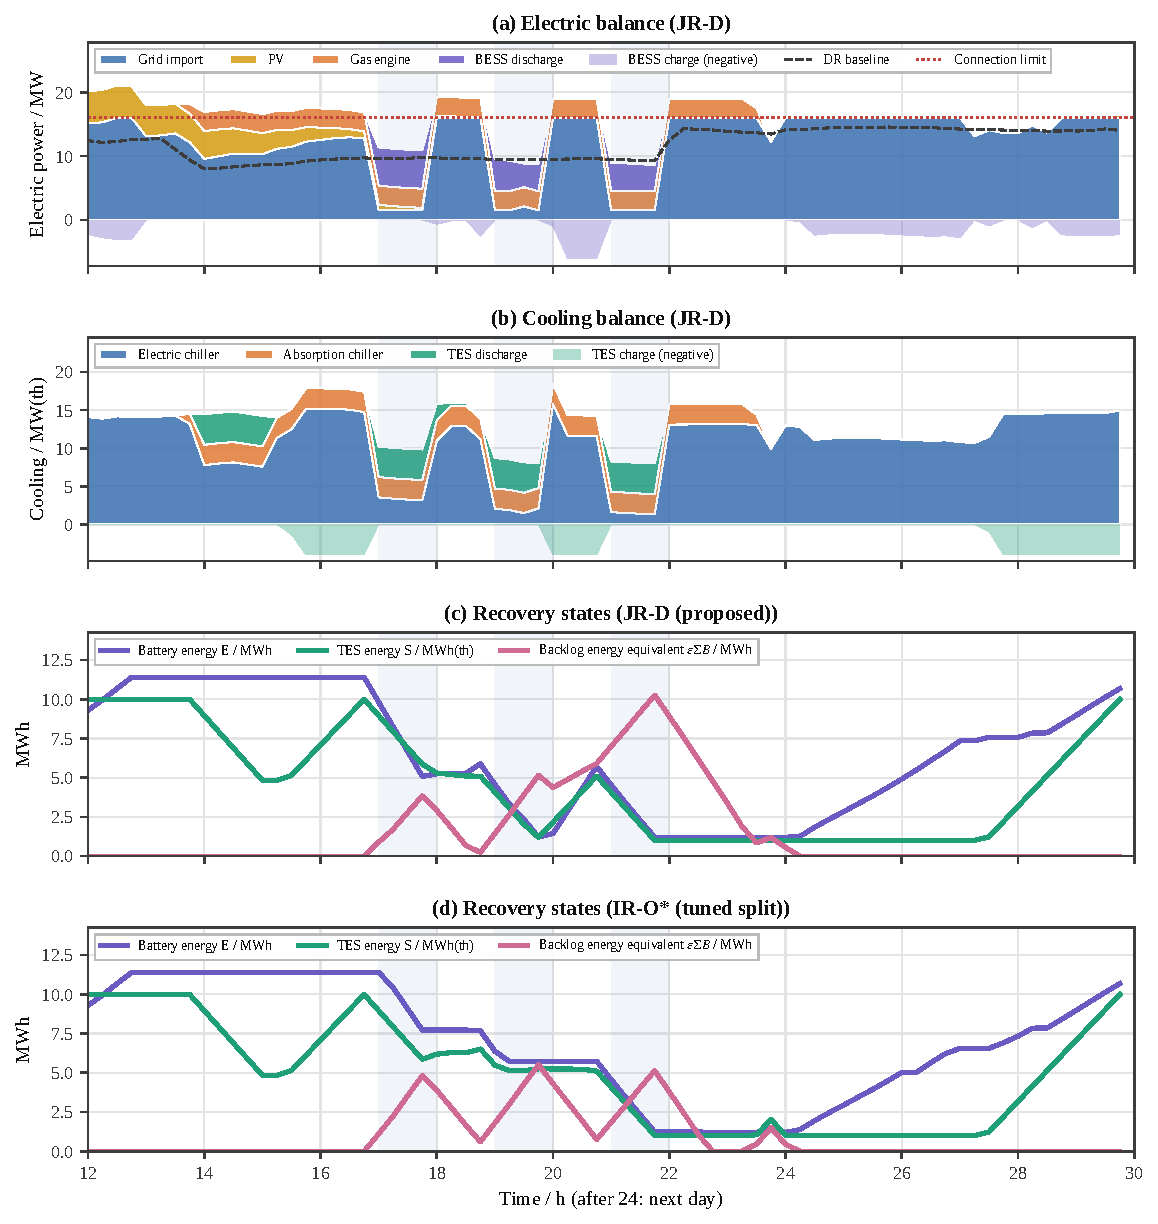
\includegraphics[width=0.80\textwidth]{fig18_typical_day.pdf}
\caption{Operation on the case day (rule setting, coupled commitment 8.18/7.98/7.90~MW). (a) Electricity balance and
(b) cooling balance of JR-D; (c)(d) recovery states of JR-D and IR-O*: BESS energy, TES energy and the electricity
equivalent of the backlog $\varepsilon\sum_cB_c$.}
\label{fig:typical}
\end{figure*}

\begin{figure*}[!t]
\centering
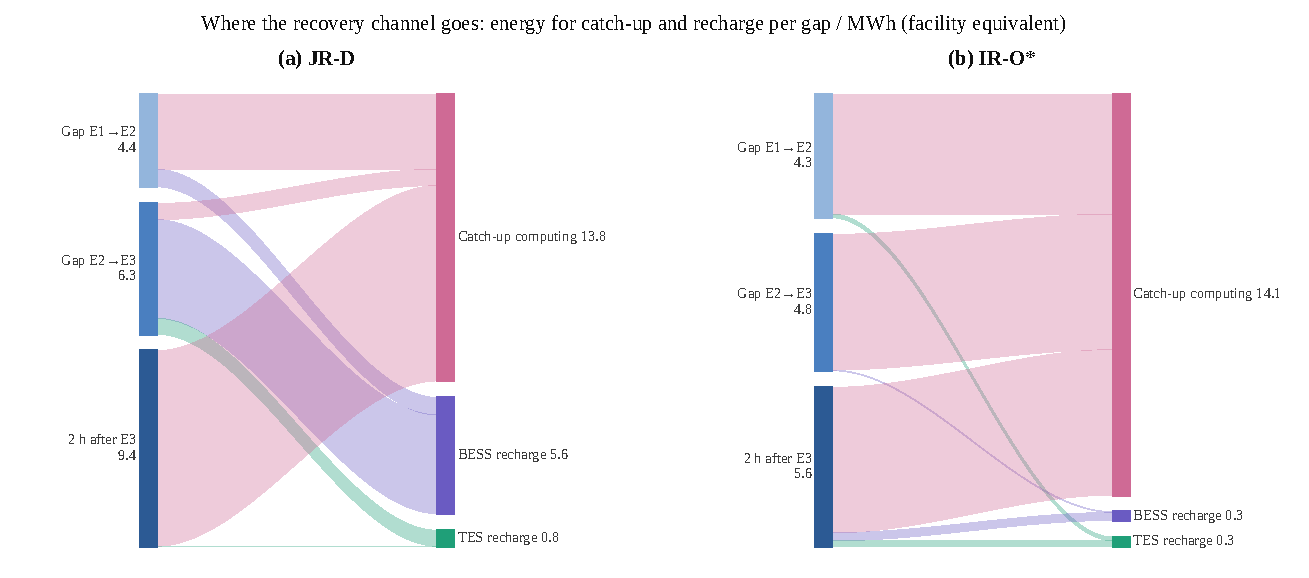
\includegraphics[width=0.78\textwidth]{fig19_channel_flows.pdf}
\caption{Use of the recovery channel in each gap and in the 2~h after E3 (same setting as \figref{fig:typical}):
energy for catch-up computing, BESS recharging and TES recharging.}
\label{fig:flows}
\end{figure*}

Joint recovery is most valuable when the commitments approach the single-event capabilities. In the rule setting with
the coupled commitment, JR-D keeps all three events valid (fulfilment 99.3\%), whereas the strongest independent
benchmark IR-O* fulfils 80.3\% and loses E2; the total cost of JR-D is 15.7\% lower than that of IR-O* and 22.5\% lower
than that of IR-P. \figref{fig:typical} and \figref{fig:flows} show why. JR-D defers more long-lag work during E2, so
that a backlog of 6,027~GPU$\cdot$h, about 10~MWh of facility electricity, is carried into E3; the channel between E2
and E3 is used mainly to recharge the BESS and TES (5.6 and 0.8~MWh), and the backlog is worked off after E3. IR-O*
spends almost the whole channel of the three gaps on catch-up computing (14.1~MWh) and recharges only 0.3~MWh of
storage; in E2 its energy management gives up validity (delivering 4.76~MW) to save the BESS for the better-paid E3,
and IR-P delivers only 3.40~MW in E2.

With moderate commitments (uniform 6~MW), IR-O* and IR-P keep all three events valid as well, and the advantage of JR-D
shrinks to 3.2\% against IR-O* in the rule setting and 3.3\% against IR-P in the rebound-priced setting. In the rebound-priced setting the
advantage comes mainly from the rebound charge: of the $-2.6\%$ and $-3.3\%$ against IR-P, only $+1.1\%$ and $-0.6\%$
remain when the rebound charge is excluded, because the charge makes the channel expensive after each event and joint
recovery moves catch-up to cheaper hours. Price coordination does not replace joint recovery: IR-P is the strongest
benchmark in the rebound-priced setting but the weakest with high commitments in the rule setting (73.7\%), because a
one-shot day-ahead price is no longer correct once the state deviates from the plan and because the non-unique LP
response lets the IT side crowd the channel again (Proposition~\ref{prop:price}). Cross-event foresight is essential:
the event-by-event JR-M fulfils 84--92\% and costs 8--19\% more than JR-D. The scenario MPC and the perfect-information
reference differ from JR-D by less than 0.5\%.

\subsubsection{Out-of-sample performance on 52 operating days}
\label{sec:res-mc}

\tabref{tab:mc} reports the 52 operating days with a uniform commitment of 6~MW for three settings, and
\figref{fig:ridge} shows the full cost distributions (the box plots are given in \figref{fig:mcbox}). The distribution
of JR-D is shifted to the left as a whole and has the shortest right tail.

\begin{table}[!t]
\caption{Out-of-sample results on 52 operating days (uniform 6~MW; means, 95\% CI in brackets).}
\label{tab:mc}
\centering\footnotesize
\setlength{\tabcolsep}{2.6pt}
\begin{tabular}{@{}lcccc@{}}
\toprule
Strategy & \makecell{Fulfilment\\(\%)} & \makecell{All\\valid} & \makecell{Max rebound\\(MW)} & \makecell{Total cost\\($10^4$~CNY)}\\
\midrule
\multicolumn{5}{@{}l}{\textit{Events certain, $\crb=3$~CNY/kW}}\\
IR-R & 71.1 [66.4, 75.7] & 11.5\% & 6.52 & 30.25 [29.18, 31.33]\\
IR-O & 81.6 [76.9, 86.2] & 48.1\% & 6.28 & 26.00 [24.91, 27.09]\\
IR-O* & 97.8 [96.5, 99.1] & 90.4\% & 6.22 & 24.30 [23.45, 25.15]\\
IR-P & 98.3 [96.7, 99.9] & 94.2\% & 5.30 & 23.20 [22.46, 23.94]\\
JR-M & 91.7 [89.6, 93.8] & 48.1\% & 6.35 & 24.81 [23.78, 25.84]\\
\textbf{JR-D} & \textbf{99.9 [99.7, 100]} & \textbf{100\%} & \textbf{4.85} & \textbf{22.53 [21.79, 23.27]}\\
\multicolumn{5}{@{}l}{\textit{Events certain, $\crb=0$ (Jiangsu settlement only)}}\\
IR-O* & 99.2 [98.5, 99.9] & 98.1\% & 6.5 & 19.71 [19.07, 20.35]\\
IR-P & 93.3 [90.7, 96.0] & 86.5\% & 6.5 & 20.21 [19.42, 20.99]\\
JR-M & 94.6 [92.5, 96.6] & 67.3\% & 6.5 & 21.38 [20.39, 22.36]\\
\textbf{JR-D} & \textbf{99.9 [99.7, 100]} & \textbf{100\%} & 6.5 & \textbf{19.10 [18.54, 19.67]}\\
\multicolumn{5}{@{}l}{\textit{E3 called with probability 0.6, confirmed 1~h ahead, $\crb=3$}}\\
IR-O* & 98.2 & 94.2\% & -- & 24.26\\
IR-P & 97.6 & 94.2\% & -- & 23.67\\
JR-M & 94.9 & 67.3\% & -- & 24.10\\
JR-D & 99.98 & 100\% & -- & 22.74\\
JR-S (scenario tree) & 99.7 & 100\% & -- & 22.65\\
JR-oracle & 100.0 & 100\% & -- & 22.27\\
\bottomrule
\end{tabular}
\end{table}

\begin{figure*}[!t]
\centering
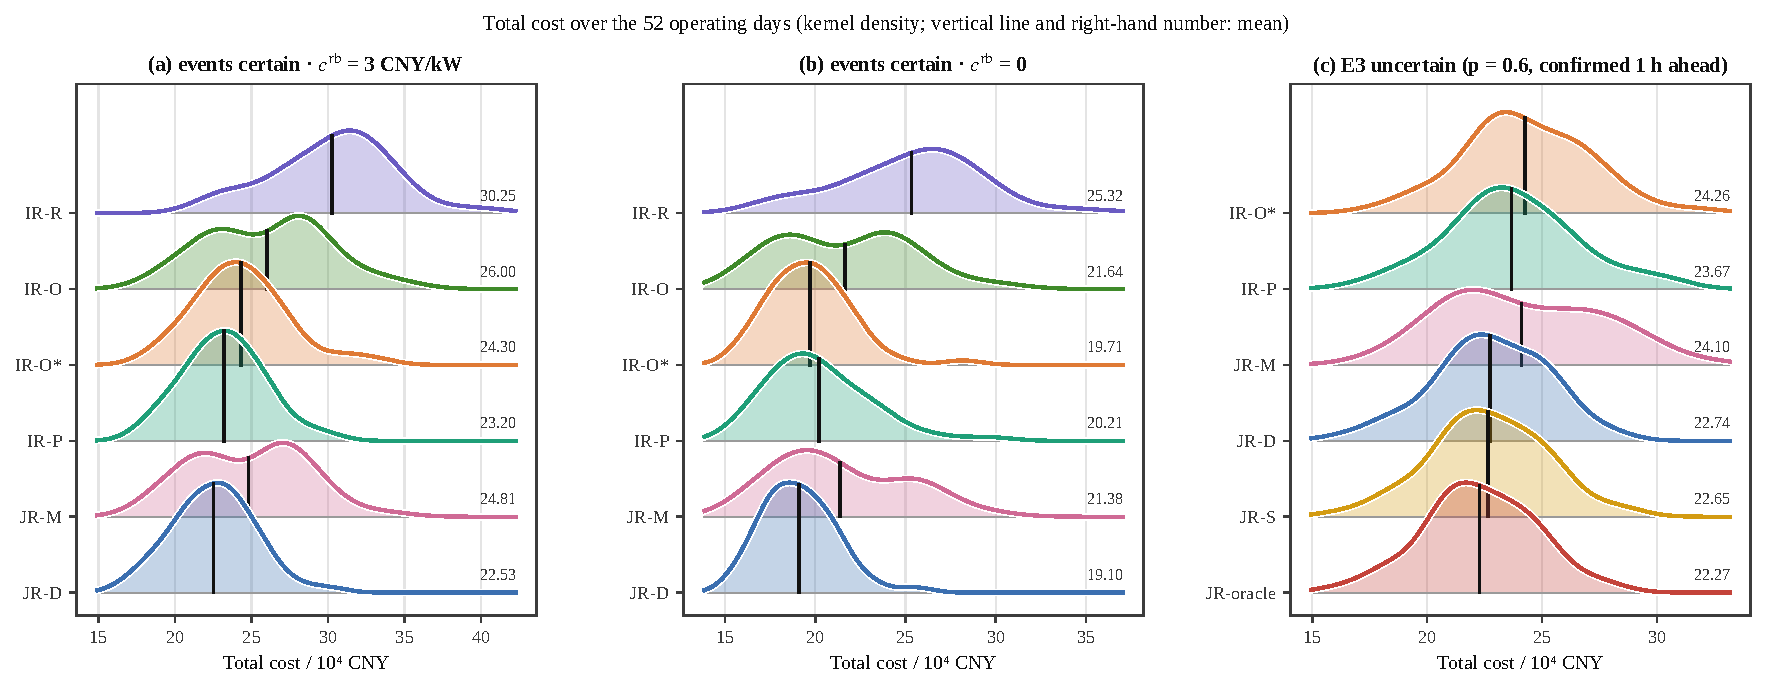
\includegraphics[width=0.94\textwidth]{fig24_ridge_montecarlo.pdf}
\caption{Kernel densities of the daily total cost on the 52 operating days for the three settings (vertical lines and
right-hand numbers: means, $10^4$~CNY).}
\label{fig:ridge}
\end{figure*}

With events certain and the rebound priced, the paired daily difference of JR-D against IR-P is $-6{,}692$~CNY per day
(95\% CI $[-7{,}891,-5{,}492]$, $-2.9\%$, $p=4\times10^{-10}$, cheaper on 50 of the 52 days), with a 8.4\% lower maximum
rebound and 1.6 percentage points higher fulfilment; against IR-O* the cost is 7.3\% lower on all 52 days and the
maximum rebound 22.0\% lower; against JR-M the cost is 9.2\% lower (52/52 days) and the fulfilment 8.2 points higher.
Excluding the rebound charge, the difference to IR-P ($-0.7\%$) is not significant ($p=0.64$), and that to IR-O* is
$+0.9\%$. In the rule setting, JR-D costs 3.1\% less than IR-O* ($-6{,}062$~CNY per day $[-7{,}053,-5{,}072]$, 52/52 days,
$p=4\times10^{-10}$) and 5.5\% less than IR-P; all strategies then raise the import to about 6.5~MW above the baseline
after the events. When E3 is uncertain, JR-D costs 4.0\% less than IR-P (51/52 days) and 6.3\% less than IR-O*. The
scenario MPC gains little: JR-S is 0.4\% cheaper than JR-D ($-821$~CNY per day $[-2{,}064,+421]$, $p=0.46$), saving
5,400~CNY on days when E3 is not called and losing 2,300~CNY on days when it is, so the scenario tree trades part of
the value of called days for a hedge against cancellation. JR-D is 2.1\% above perfect information, mostly because of
the rebound charge (0.2\% without it, $p=0.43$). In summary, against the strongest benchmark of each setting, joint
recovery is 2.9--4.0\% cheaper and keeps all events valid on every day, whereas the benchmarks achieve this on 86--98\%
of the days.

\subsubsection{Sources of benefit and contribution of the mechanisms}
\label{sec:res-sources}

\tabref{tab:ablation} isolates the resources (uniform 6~MW, $\crb=3$, perfect information). Without computing
flexibility ($L=0$) the two strategies are identical: with a single recovery state there is nothing to coordinate. Even
with the hindsight-optimal static split ($\alpha^*=0.9$, fulfilment 100\%), joint recovery is still 6.9\% cheaper.

\begin{table}[!t]
\caption{Ablation (uniform 6~MW, $\crb=3$, perfect information; fulfilment / total cost in $10^4$~CNY).}
\label{tab:ablation}
\centering\footnotesize
\begin{tabular}{@{}lccc@{}}
\toprule
Configuration & IR-O & JR & JR vs IR-O\\
\midrule
Full system & 89.2\% / 25.58 & 100\% / 22.80 & $-10.9\%$\\
No computing flexibility ($L=0$) & 29.0\% / 28.72 & 29.0\% / 28.72 & 0\\
No BESS & 16.4\% / 35.54 & 36.1\% / 32.38 & $-8.9\%$\\
No TES & 68.1\% / 27.03 & 100\% / 23.49 & $-13.1\%$\\
IR-O with hindsight split $\alpha^*=0.9$ & 100\% / 24.49 & -- & $-6.9\%$\\
\bottomrule
\end{tabular}
\end{table}

\begin{figure*}[!t]
\centering
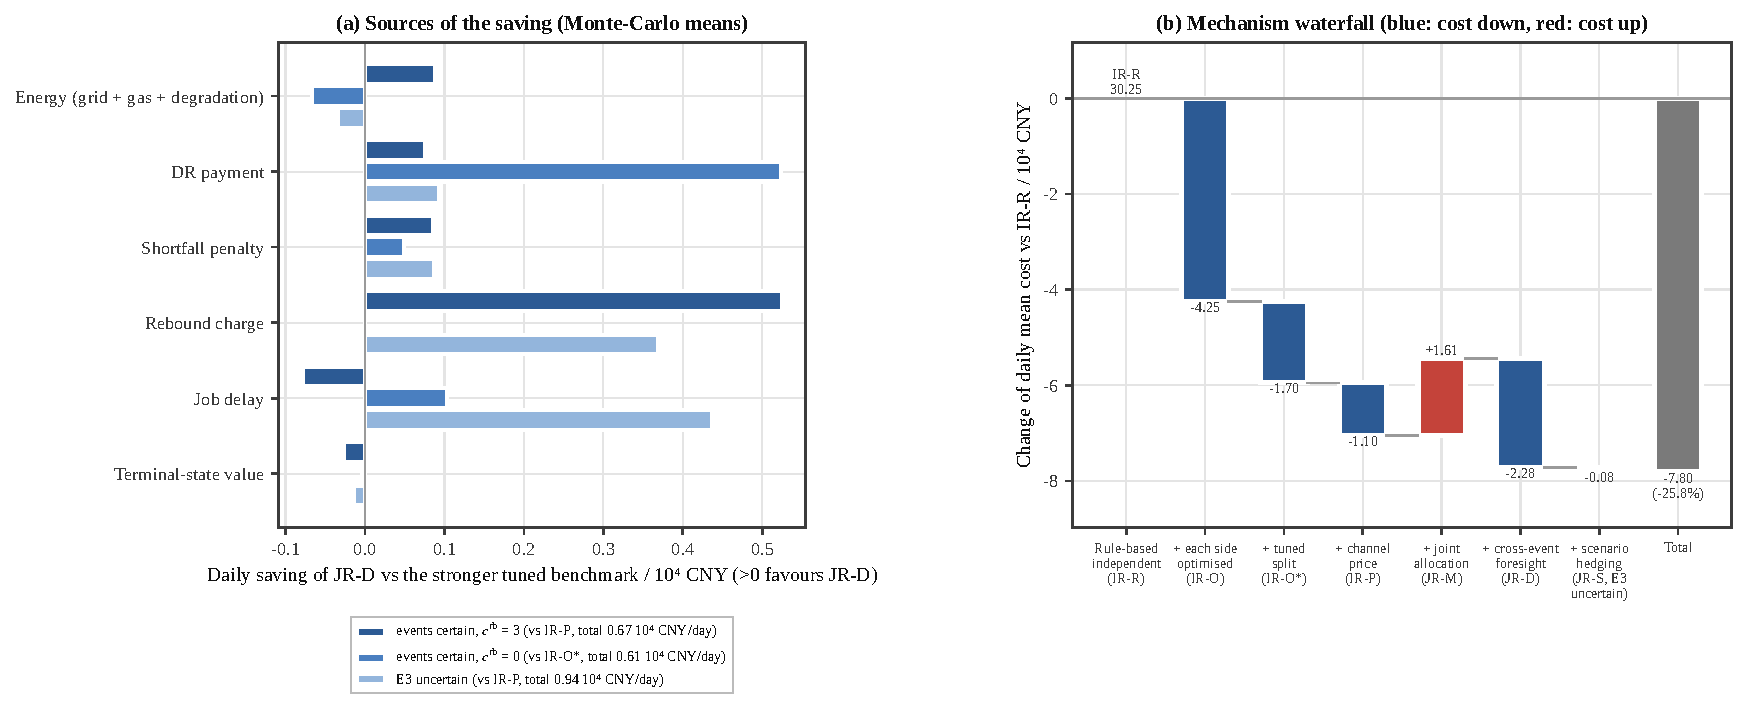
\includegraphics[width=0.94\textwidth]{fig16_decomposition.pdf}
\caption{(a) Daily saving of JR-D against the stronger tuned benchmark, decomposed by source (means over the 52 days);
(b) contribution of each coordination mechanism, starting from rule-based independent recovery (events certain,
$\crb=3$; the last step uses the uncertain-E3 setting).}
\label{fig:decomp}
\end{figure*}

\figref{fig:decomp}(b) adds one coordination mechanism at a time to the rule-based IR-R (30.25$\times10^4$~CNY per day):
optimising each side ($-4.25$), tuning the split on history ($-1.70$), sending the channel price ($-1.10$), allocating
the channel jointly but event by event ($+1.61$), adding cross-event foresight ($-2.28$) and hedging the uncertain event
by scenarios ($-0.08$), a total of $-7.80\times10^4$~CNY ($-25.8\%$). Optimising each side and cross-event foresight
contribute most. Joint allocation without foresight (JR-M) is worse than price coordination, because after each event it
catches up or recharges as if only one more event followed and often spends the channel on the wrong state; joint
allocation and cross-event foresight are both needed.

\figref{fig:decomp}(a) decomposes the daily saving of JR-D against the stronger benchmark. With the rebound priced, 78\%
of the saving of $0.67\times10^4$~CNY against IR-P comes from the rebound charge. In the rule setting, 86\% of the
saving of $0.61\times10^4$~CNY against IR-O* comes from the additional DR payment of keeping all three events valid.
When E3 is uncertain, the largest item is the job-delay cost ($0.44$ of $0.94\times10^4$~CNY), because the IT side of
IR-P follows the day-ahead price and defers too much while the call of E3 is unknown. The energy cost hardly changes in
any setting: joint recovery does not save money by more arbitrage.
